%!TEX root = ../main.tex

\thispagestyle{empty}
\vspace{-0.7cm}

\cleanchapterquote{Es precipitado afirmar que un teorema matemático no puede demostrarse de una manera particular; pero algo parece bastante claro... tenemos ciertas ideas sobre la lógica de la teoría; creemos que algunos teoremas, como solemos decir, “yacen profundamente” y otros están más cerca de la superficie. Si alguien produce una demostración elemental del teorema de los números primos, mostrará que estas ideas son erróneas, que el tema no se sostiene de la manera que habíamos supuesto, y que es hora de desechar los libros y reescribir la teoría.}{Godfrey Harold Hardy (1921)
}{\textit{Conferencia a la Sociedad Matemática de Copenhague}}

Obtener cotas, tanto superiores como inferiores, para la función contadora de primos $\pi(x)$ es un desafío notablemente difícil. En vista de estas dificultades, es excepcional que a mediados del siglo XIX, el matemático ruso P. L. Chebyshev lograra determinar el orden preciso de magnitud de $\pi(x)$. Chebyshev demostró que existen constantes positivas $A$ y $B$ tales que

$$
A \frac{x}{\log x} \leq \pi(x) \leq B \frac{x}{\log x}
$$


para valores de $x$ suficientemente grandes. De hecho, obtuvo las cotas específicas de $A\approx 0,92129$ y $B=(6/5) A \approx 1,10555$, esto le permitió demostrar el Postulado de Bertrand, que establece que para $x>2$, siempre existe un número primo $p$ tal que $x<p<2 x$, además demostró que si $\pi(x)/(x\log x)$ tenía un límite cuando $x\to \infty$, entonces este límite tenía que ser 1.\\

El método de Chevyshev consistía en explotar el TFA para convoluciones 

$$\sum_{j \mid n}\Lambda(j)=\log n,$$

para realizar estimaciones sobre las sumas parciales del logaritmo natural, esto es $\log([x]!)$, en retrospectiva la aproximación de Chebyshev se basa en la relación

\[
[x] = \prod_{p} p^{\nu_p([x])}, \quad \text{donde } \nu_p([x]) \text{ es el orden } p\text{-ádico}
\]


 de esta identidad se puede comparar la valuación $p$-ádica con la arquimediana, muchos intentos de producir una prueba usando estos métodos fallaron, el teorema se resistió a una prueba elemental por lo siguientes cien años.\\

Años después, en 1859, aparece el famoso artículo de Riemann ``Sobre la cantidad de primos menores que una magnitud dada'', allí se encontraba el camino hacia una prueba del TNP. La idea revolucionaria de Riemann fue considerar a $\zeta(s)$ como una función de variable compleja y expresar a $\pi(x)$ en términos de una integral compleja que involucraba a $\zeta(s)$, más aún, Riemann obtiene la fórmula explícita

$$\pi(x)=\operatorname{Li}(x)-\sum_\rho \operatorname{Li}\left(x^\rho\right)-\log (2)+\int_x^{\infty} \frac{d t}{t\left(t^2-1\right) \log (t)},$$

en donde $\rho$ denota un cero no trivial de la función $\zeta(s)$, sin embargo, no había suficiente análisis disponible para producir una prueba rigurosa. No fue hasta finales del siglo XIX cuando se proporcionó el ingrediente esencial que faltaba, este fue la teoría de las funciones enteras de orden finito, desarrollada por Hadamard para probar el TNP.\\

Riemann demostró que la función $\zeta(s)$ tiene una continuación analítica a $\C$ excepto por un polo simple en $s=1$ con residuo 1 y además obtuvo su ecuación funcional 

\[
\zeta(s) = 2^s \pi^{s-1} \sin\left(\frac{\pi s}{2}\right) \Gamma(1-s) \zeta(1-s),
\]

también reconoció el papel importante que juegan los ceros de $\zeta(s)$ en la teoría de números y conjetura varias propiedades de estos ceros, todas estas conjeturas excepto una fueron demostradas por Von Mangolth y Hadamard a finales del siglo XIX, la conjetura que se resistió es la ya muy famosa hipótesis de Riemann ``la parte real de todos los ceros no triviales de $\zeta(s)$ es 1/2'', al conjeturarla, Riemann dice ``es muy probable que ...'' (es ist sehr wahrscheinlich dass).\cite{bateman1996hundred}\\

En 1896 aparecen las pruebas de Hadamard y Charles-Jean de La Vallée Poussin, ambos prueban que $\zeta(1+it)\neq 0$ para todo $t\in \R$, esto es que la función $\zeta(s)$ no se anula en los complejos con parte real 1, esto les permite dar una prueba rigurosa siguiendo las ideas de Riemann, dicho esto, las pruebas de Hadamard y de la Vallée Poussin requieren análisis de la función zeta en una franja más grande que simplemente $\Re(s)\geq 1$ dado que involucran fórmulas explícitas en la prueba y en estas los ceros de $\zeta(s)$ juegan un papel importante.\\

En este capítulo veremos que el TNP implica que $\zeta(s)\neq 0$ para $\Re(s)=1$, esto ya era conocido por los matemáticos de la época y nos dice que es necesaria la no nulidad en la recta vertical para obtener el teorema de los números primos, el primer matemático en dar una prueba que no dependía de la ecuación funcional de $\zeta(s)$ fue Landau, en su lugar trabaja con la extensión analítica en el semiplano $\Re(s)>0$ que estudiamos previamente.

La pregunta natural que surge aquí es ¿puede el teorema de los números primos ser probado usando solo el hecho de que $\zeta(s)\neq 0$ en $\Re(s)=1$?, la respuesta fue dada por N. Wiener en 1931 con su famoso teorema Tauberiano


\begin{theorem}
Sean $a_n \geq 0$ y $F(s)=\displaystyle\sum_{n=1}^{\infty} \frac{a_n}{n^s}$ una serie absolutamente convergente. Supongamos que se cumplen las siguientes condiciones:

\begin{itemize}
\item[a)] La función $F(s)$ se extiende a una función analítica en la región $\Re(s) \geq 1$ con un único polo simple en $s=1$, cuyo residuo es $1$.
\item[b)] $A(x)=\displaystyle \sum_{n \leq x} a_n=O(x)$.
\end{itemize}


Entonces, se tiene que

$$
A(x)=x+o(x) \text { cuando } x \rightarrow \infty \text {. }
$$
\end{theorem}

De este teorema el TNP resulta ser un corolario, más aún, obtenemos una equivalencia entre el teorema de los números primos y $\zeta(1+it)\neq 0$ ya que como podemos ver en las condiciones del teorema, no requerimos análisis por fuera de la franja $\Re(s)\geq 1$ y esta dirección será la que tomaremos en este trabajo.

\section{El teorema de Wiener-Ikehara}

Sea $\displaystyle \sum_{n=0}^{\infty} a_n x^n$, $x\in \R$ una serie de potencias centrada en $0$ y con radio  de convergencia $1$, en el borde la región, la serie puede ser divergente o convergente. El teorema de Abel nos dice que si la serie es sumable en un punto del borde, entonces es continua en el punto, más precisamente, si
$$\sum_{n=0}^{\infty} a_n=A,$$
entonces
$$\lim_{x \to 1^-}\sum_{n=0}^{\infty} a_n x^n=A.$$

Uno podría preguntarse cuando esperar un recíproco de este teorema, bajo qué condiciones que este límite tenga cierto valor $A$, implica que la serie es sumable y converge a $A$, las primeras condiciones fueros establecidas por Tauber

\begin{prop}[Tauber, 1897]
    Sea $f(x)=\displaystyle\sum_{n=0}^{\infty} a_n x^n$ una serie de potencias que converge absolutamente para $|x|<1$.
Si $\lim_{x \rightarrow 1^{-}} f(x)=A$ y se cumple la condición $a_n=o\left(\dfrac{1}{n}\right)$, entonces $f(1)=A$.
\end{prop}

Los teoremas tauberianos son recíprocos condicionales del teorema de Abel, la condición $a_n=o\left(\dfrac{1}{n}\right)$ nos restringe el crecimiento de los coeficientes, estas condiciones fueron relajadas subsecuentemente por Hardy y Littlewood a $O\left(\dfrac{1}{n}\right)$ y posteriormente a $na_n>-K$.\\

Algunas de las aplicaciones más importantes de la teoría tauberiana son a la teoría analítica de números, en este contexto los resultados tauberianos se pueden considerar como estimaciones sobre las sumas parciales de los coeficientes de una serie de Dirichlet.

En 1980 el matemático Donald J. Newman dió una prueba corta del teorema de los números primos, utilizando el siguiente teorema tauberiano

\begin{theorem}[Newman]
    Supongamos que 

    $$|a_n|\leq 1 \text{ y } F(s)=\sum_{n=1}^{\infty} \frac{a_n}{n^s}.$$

    Entonces $F$ es analítica en el semiplano $\sigma>1$. Si $F$ tiene extensión analítica en el semiplano $\sigma\geq 1$, entonces $\displaystyle\sum_{n=1}^{\infty} \frac{a_n}{n^s}$ converge en $\sigma\geq 1$.
\end{theorem}

La prueba de Newman inspiró dos grandes artículos que modificaron su prueba, los de Zagier \cite{zagier1997newman} y Korevaar \cite{korevaar1982newman}, en donde se aprovecha la relación que hay entre transformada de Laplace y series de Dirichlet, esto nos permite dar una prueba del TNP en la que solo se emplea el teorema de residuos de Cauchy.\\

En esta sección presentaremos una prueba del teorema de Wiener-Ikehara modificando la prueba de Newman, esto es, siguiendo el enfoque de Zagier y Korevaar de una manera distinta, este camino para la prueba fue encontrado por Korevaar \cite{korevaar2006wiener}, también presentaremos versiones más fuertes del teorema siguiendo a \cite{vatwani2015simple}, estas versiones son las que necesitaremos para el TNP en progresiones aritmética del siguiente capítulo.

\begin{theorem}[Korevaar y Zagier]
    Para $t \geq 0$, sea $f(t)$ una función acotada y localmente integrable y sea $$g(s):=\displaystyle\int_0^{\infty} f(t) e^{-s t} d t,$$
     para $\Re(s)>0$. Si $g(s)$ tiene continuación analítica a $\Re(s) \geq 0$, entonces $\displaystyle\int_0^{\infty} f(t) d t$ existe y es igual a $g(0)$.
\end{theorem}

\begin{proof}
    Dado $T>0$, sea

    $$g_T(s)=\int_0^Tf(t)e^{-st}dt,$$

    por hipótesis $g_T(s)$ converge para todo $s\in \C$, y $g_T(s)$ es una función entera, queremos ver que 

    $$\lim_{T \to \infty} \int_0^T f(t)dt=g(0).$$
 
    Dado $R>0$, considere el siguiente contorno positivamente orientado $\mathscr{C}$

    \begin{center}
    %!TEX root = ../main.tex

\tikzset{every picture/.style={line width=1pt}} %set default line width to 0.75pt        

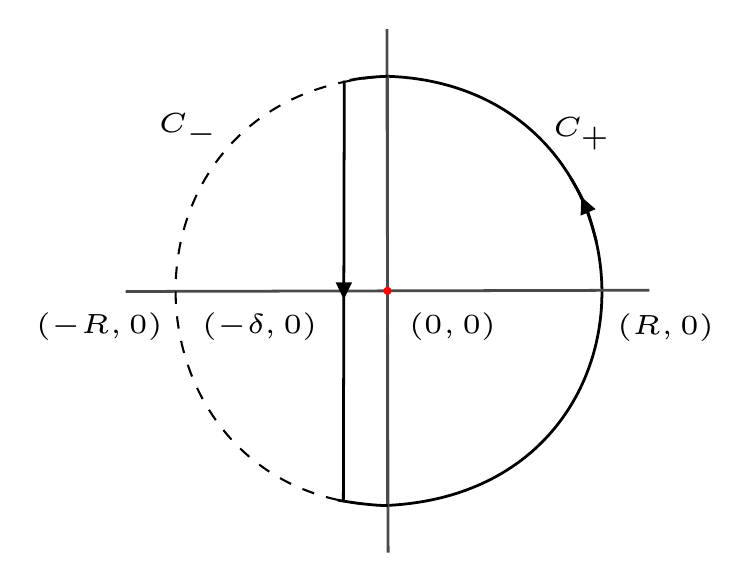
\begin{tikzpicture}[x=0.86pt,y=0.86pt,yscale=-1,xscale=1]
%uncomment if require: \path (0,357); %set diagram left start at 0, and has height of 357

%Curve Lines [id:da6356687025771366] 
\draw    (275.97,140.51) .. controls (393.49,144.53) and (398.68,314.72) .. (275.97,320.82) ;
%Straight Lines [id:da7778166164432772] 
\draw [color={rgb, 255:red, 74; green, 74; blue, 74 }  ,draw opacity=1 ]   (165.97,230.93) -- (385.97,230.41) ;
%Straight Lines [id:da7053132902182386] 
\draw [color={rgb, 255:red, 74; green, 74; blue, 74 }  ,draw opacity=1 ]   (276.23,340.67) -- (275.71,120.67) ;
%Straight Lines [id:da3860117988849814] 
\draw [color={rgb, 255:red, 74; green, 74; blue, 74 }  ,draw opacity=1 ]   (275.97,140.51) -- (275.97,320.82) ;
%Curve Lines [id:da8696519251258394] 
\draw [line width=0.75]  [dash pattern={on 4.5pt off 4.5pt}]  (275.97,320.82) .. controls (161.04,319.39) and (153.49,147.13) .. (275.97,140.51) ;
%Straight Lines [id:da885594660241974] 
\draw    (257.81,142.33) -- (257.42,318.61) ;
\draw [shift={(257.61,234.27)}, rotate = 270.13] [fill={rgb, 255:red, 0; green, 0; blue, 0 }  ][line width=0.08]  [draw opacity=0] (7.14,-3.43) -- (0,0) -- (7.14,3.43) -- cycle    ;
%Curve Lines [id:da01957205219237279] 
\draw    (260.05,142.23) .. controls (265.49,141.06) and (271.33,140.68) .. (275.97,140.51) ;
%Curve Lines [id:da7685319347743758] 
\draw    (275.97,320.82) .. controls (271.82,321.03) and (262.09,319.86) .. (255.08,318.61) ;
%Curve Lines [id:da9382254876031242] 
\draw    (352.85,183.1) .. controls (360.63,195.56) and (361.15,201.09) .. (363.74,209.91) ;
\draw [shift={(357.4,191.16)}, rotate = 66.46] [fill={rgb, 255:red, 0; green, 0; blue, 0 }  ][line width=0.08]  [draw opacity=0] (7.14,-3.43) -- (0,0) -- (7.14,3.43) -- cycle    ;
%Shape: Ellipse [id:dp016643737096258437] 
\draw  [color={rgb, 255:red, 255; green, 0; blue, 0 }  ,draw opacity=1 ][fill={rgb, 255:red, 255; green, 0; blue, 0 }  ,fill opacity=1 ] (274.86,230.67) .. controls (274.86,230.05) and (275.36,229.56) .. (275.97,229.56) .. controls (276.58,229.56) and (277.08,230.05) .. (277.08,230.67) .. controls (277.08,231.28) and (276.58,231.78) .. (275.97,231.78) .. controls (275.36,231.78) and (274.86,231.28) .. (274.86,230.67) -- cycle ;

% Text Node
\draw (125.36,236.93) node [anchor=north west][inner sep=0.75pt]  [font=\normalsize,xscale=2,yscale=2]  {\fontsize{4}{4}\selectfont$(-R,0)$};
% Text Node
\draw (282.08,236.93) node [anchor=north west][inner sep=0.75pt]  [font=\tiny,xscale=2,yscale=2] [align=left] {\fontsize{4}{4}\selectfont$( 0,0)$};
% Text Node
\draw (195.08,236.93) node [anchor=north west][inner sep=0.75pt]  [font=\tiny,xscale=2,yscale=2] [align=left] {\fontsize{4}{4}\selectfont$(-\delta,0)$};
% Text Node
\draw (369,236.93) node [anchor=north west][inner sep=1pt]  [font=\tiny,xscale=2,yscale=2]  {\fontsize{4}{4}\selectfont$(R,0)$};
% Text Node
\draw (342.5,154.9) node [anchor=north west][inner sep=0.75pt]  [font=\tiny,xscale=2,yscale=2]  {$\mathscr{C}_{+}$};
% Text Node
\draw (176.83,153.4) node [anchor=north west][inner sep=0.75pt]  [font=\tiny,xscale=2,yscale=2]  {$C_{-}$};

\end{tikzpicture}
    \end{center}

    donde $\delta>0$ (dependiendo de $R$) se escoge de tal forma que $g(s)$ es analítica en $\mathscr{C}$, esto se puede hacer ya que el conjunto $A:=\{(0,y): y\in [-R,R]\}$ es compacto y como $g(s)$ es analítica, $A$ se puede cubrir por bolas abiertas, en cada una de las cuales $g(s)$ es analítica, la compacidad permite escoger un subcubrimiento finito, del que obtenemos $\delta$.  Denotemos

    $$\mathscr{C}_+=\mathscr{C}\cap \{s:\sigma>0\},\quad \quad \mathscr{C}_-=\mathscr{C}\cap \{s:\sigma<0\}$$

    y como $C_-$ el semicírculo de radio $R$ a la izquierda de $\sigma=0$, aplicando fórmula de la integral de Cauchy obtenemos que

    $$I_{\mathscr{C}}=\frac{1}{2\pi i}\int_{\mathscr{C}}\left(g(s)-g_T(s)\right)e^{sT}\left(1+\frac{s^2}{R^2}\right)\frac{1}{s}ds=g(0)-g_T(0)$$

    dado que todas las funciones en la integral $I_{\mathscr{C}}$ son analíticas, excepto por $1/s$ que tiene un polo simple en $s=0$, de donde obtenemos el residuo $g(0)-g_T(0)$.\\

    Sea $M = \sup _{t \geq 0}|f(t)|$. En $\mathscr{C}_{+}$, dado que $\sigma > 0$, tenemos

\[
\left|g(s)-g_T(s)\right| = \left|\int_T^{\infty} f(t) e^{-s t} d t\right| \leq M \int_T^{\infty} e^{-\sigma t} d t \ll \frac{e^{-\sigma T}}{\sigma}.
\]

Tomando $s = R e^{i \theta}$, entonces $R \cos \theta = \sigma$ en $\mathscr{C}_{+}$, obtenemos la siguiente estimación:

\begin{equation}
    \begin{aligned}
    \left|e^{s T} \frac{1}{s}\left(1+\frac{s^2}{R^2}\right)\right| &= e^{\sigma T}\left|\frac{1}{R e^{i \theta}}+\frac{e^{i \theta}}{R}\right|\\
    &=e^{\sigma T}\left|\frac{e^{-i\theta}+e^{i\theta}}{R}\right|\\
    &=e^{\sigma T}\left|\frac{2 \cos \theta}{R}\right| \ll e^{\sigma T} \frac{|\sigma|}{R^2},
\end{aligned}
\end{equation}

por lo tanto, acotando en la integral obtenemos que

\[
\left|I_{\mathscr{C}_{+}}\right| \ll \frac{1}{R^2}\left|\int_{\mathscr{C}_{+}} d s\right|=\frac{1}{R^2}\pi R\ll \frac{1}{R}.
\]

En $\mathscr{C}_{-}$, examinamos $g_T(s)$ y $g(s)$ por separado. Consideremos primero la integral

\[
I_1 := \frac{1}{2 \pi i} \int_{\mathscr{C}_{-}} g_T(s) e^{s T}\left(1+\frac{s^2}{R^2}\right) \frac{d s}{s}.
\]

Como $g_T(s)$ es entera y el resto del integrando es analítico a la izquierda de $\sigma = 0$, tenemos que

\[
I_1 = \frac{1}{2 \pi i} \int_{C_{-}} g_T(s) e^{s T}\left(1+\frac{s^2}{R^2}\right) \frac{d s}{s}.
\] 

Es decir, podemos integrar sobre el semicírculo \( C_{-} \) en lugar de \( \mathscr{C}_{-} \), con \( C_{-} \) orientado de la misma manera que \( \mathscr{C}_{-} \). Luego, observando que \( \sigma < 0 \) en este caso, tenemos  

\[
\left|g_T(s)\right| = \left|\int_0^T f(t) e^{-s t} d t\right| \leq M \int_0^T e^{-\sigma t} d t \ll \frac{e^{-\sigma T}}{|\sigma|}.
\]

La estimación en (3.1) sigue siendo válida, por lo que de manera análoga obtenemos que

$$|I_{1}|\ll \frac{1}{R},$$

nos queda acotar la integral restante

$$I_2=\frac{1}{2\pi i }\int_{\mathscr{C}_-}g(s)e^{st}\left(1+\frac{s^2}{R^2}\right)\frac{1}{s}ds.$$

Como $\mathscr{C}_-$ está contenido en un compacto en el que $g(s)$ es analítica, $|g(s)|$ se puede acotar por una constante que depende únicamente de $R$, digamos 

$$|g(s)|\leq M_R,$$

para todo $s \in \mathscr{C}_-$, $s=e^{i\theta}$ o $s=-\delta+it$, esto es, $s$ está en los arcos de circunferencia, o $s$ está en la recta vertical $\Re(s)=-\delta$, debemos acotar la integral en estos dos caminos del contorno, para $s=e^{i\theta}$ ya tenemos una cota dada por (3.1), si $s=-\delta+it$ tenemos que

\begin{align*}
    \left|\frac{e^{s T}}{s}\left(1+\frac{s^2}{R^2}\right)\right|&\leq \frac{e^{-\delta T}}{|s|}\left(1+\frac{|s|^2}{R^2}\right)\\
    &\leq e^{-\delta T}\left(\frac{1}{|s|}+\frac{|s|}{R^2}\right)\\
    &\leq e^{-\delta T}\left(\frac{1}{\delta}+\frac{1}{R}\right)
,\end{align*}

ya que $|t|\leq R$, combinanto esta cota junto con (3.1) y sabiendo que $|g(s)|\leq M_R$, podemos acotar la integral como

$$|I_2|\ll \frac{M_R}{R^2}\left|\int_{\mathscr{C}_-} |\sigma|e^{\sigma T} d s\right|+\frac{R M_R e^{-\delta T}}{\delta}+M_R e^{-\delta T},$$


por lo tanto

\begin{equation}
    \begin{aligned}
    |g(0)-g_T(0)|&=|I_{\mathscr{C}}|\leq |I_{\mathscr{C}_+}|+|I_1|+|I_2|\\
    &\ll \frac{1}{R}+\frac{M_R}{R^2}\left|\int_{\mathscr{C}_-} |\sigma|e^{\sigma T} d s\right|+\frac{R M_R e^{-\delta T}}{\delta}+M_R e^{-\delta T}
.\end{aligned}
\end{equation}

En \( C_{-} \), tenemos \( \sigma < 0 \) y \( |\sigma| e^{\sigma T} \rightarrow 0 \) uniformemente en \( C_{-} \) cuando \( T \rightarrow \infty \). Por lo tanto, cuando \( T \rightarrow \infty \), el lado derecho de (3.2) converge a \( \dfrac{1}{R} \). Luego, tomando \( R \rightarrow \infty \), obtenemos 

\[
g(0) = \lim _{T \rightarrow \infty} g_T(0).
\]
\end{proof}

\begin{lemma}[Korevaar  y Zagier]

Sean $a_n\geq 0$ y $A(x)=\displaystyle\sum_{n\leq x} a_n$, si  la integral

$$\int_1^{\infty}\frac{A(x)-x}{x^2}dx$$

converge, entonces $A(x)\thicksim x$

\end{lemma}

\begin{proof}
    Supongamos que $A(x)\not\thicksim x$, entonces existe una constante $\lambda>1$ (o $\lambda<1$) tal que $A(x)\geq \lambda x$ (o $A(x)\leq \lambda x$) para infinitos valores de $x\to \infty$.\\

    Sin pérdida de generalidad consideramos el caso \( \lambda > 1 \). Dado que \( A(x) \) es una función creciente, se sigue que para cualquiera de los valores de \( x \) con \( A(x) \geq \lambda x \) y para \( x \leq t \leq \lambda x \), tenemos \( A(t) \geq A(x) \geq \lambda x \) y  

\[
\begin{aligned}
\int_x^{\lambda x} \frac{A(t)-t}{t^2} d t & \geq \int_x^{\lambda x} \frac{\lambda x-t}{t^2} d t = \int_1^\lambda \frac{\lambda x-v x}{(v x)^2} x d v \\
& = \int_1^\lambda \frac{\lambda-v}{v^2} d v\\
&=c(\lambda)
\end{aligned}
\]

que es una constante positiva que depende únicamente de \( \lambda \). Por lo tanto  

\[
\left|\int_x^{\infty} \frac{A(t)-t}{t^2} d t - \int_{\lambda x}^{\infty} \frac{A(t)-t}{t^2} d t\right| =c(\lambda),
\]

sin embargo, las integrales anteriores son colas de una integral convergente, por lo que ambas convergen a cero cuando \( x \rightarrow \infty \), esto contradice que $c(\lambda)>0$.\\
\end{proof}

Con esto ya podemos presentar una prueba del teorema de Wiener-Ikehara.\\

\begin{proof}\textit{ Teorema 3.1}. Tenemos, para $\Re(s)>1$ que
\[
F(s)=\sum_{n=1}^{\infty}a_nn^{-s} =s \int_1^{\infty}\frac{A(t)}{t^{s+1}} d t,
\]

Esto implica que en el semiplano \( \sigma > 1 \), \(\displaystyle \sum_{n=1}^{\infty} a_n n^{-s} \) converge absolutamente, \( F(s) \) es analítica y  

\[
F(s) - \frac{s}{s-1} = s \int_1^{\infty} \frac{A(t)-t}{t^{s+1}} d t.
\]

Cambiando \( s \) por \( s+1 \) y \( t = e^u \) en la integral, tenemos para \( \Re(s) > 0 \),  

\[
F(s+1) - 1 - \frac{1}{s} = (s+1) \int_0^{\infty} \frac{A\left(e^u\right) - e^u}{e^u} e^{-u s} d u.
\]

Por hipótesis \( A\left(e^u\right) = O\left(e^u\right) \), se sigue que la función \( f \) dada por  

\[
f(u) = \frac{A\left(e^u\right) - e^u}{e^u}
\]

es acotada en \( [0, \infty) \) e integrable en cada subintervalo cerrado y acotado de \( [0, \infty) \), y  

\begin{align}
    \frac{F(s+1) - 1 - \frac{1}{s}}{s+1} = \int_0^{\infty} f(u) e^{-s u} d u.
\end{align}

El lado izquierdo en (3.3) es analítico para \( \sigma > 0 \). Como \( F(s+1) \) tiene un polo simple en \( s = 0 \), vemos que

 \[ F(s+1) - \dfrac{1}{s}\]

 es analítica en \( s = 0 \), y para todo \( s \) con \( \sigma \geq 0 \). Por lo tanto, podemos aplicar el teorema 3.4 para obtener que la integral  

\[
\int_0^{\infty} \frac{A\left(e^u\right) - e^u}{e^u} d u = \int_1^{\infty} \frac{A(t)-t}{t^2} d t
\]

converge. Por el lema anterior, obtenemos que \( A(x) \sim x \).\\
\end{proof}

\begin{note}
    En esta prueba del teorema de Wiener-Ikehara, la idea principal fue la introducción de un kernel en la integral $I_{\mathscr{C}}$, a saber,

    $$\displaystyle \left(1+\frac{s^2}{R^2}\right)\frac{1}{s}.$$

    Esta función tiene la característica de tener un polo en $s=0$, se sigue que

    $$I_{\mathscr{C}}=\frac{1}{2\pi i}\int_{\mathscr{C}}\left(g(s)-g_T(s)\right)e^{sT}\left(1+\frac{s^2}{R^2}\right)\frac{1}{s}ds=g(0)-g_T(0),$$

    esta expresión nos permite ver que $\lim_{T \to \infty} g_T(0)=g(0)$ acotando de manera adecuada los términos en la integral y tomando el límite.\\

    Si revisamos pruebas clásicas del teorema, por ejemplo la que se encuentra en \cite{murty2007problems}, notaremos que aquí esta función juega un papel similar al del kernel de Fejér, las ideas subyacentes de las pruebas son muy similares ya que si tomamos $s=\sigma+it$, la expresión (3.3) toma la forma de una trasformada de Fourier.\\

\end{note}

Con este teorema, podemos obtener una prueba del TNP, sin embargo, en progresiones aritmética la serie de Dirichlet 

$$L(\chi,s)=\sum_{n=1}^{\infty} \frac{\chi(n)}{n^s}$$

no cumple la hipótesis $\chi(n)\geq 0$ del teorema de Wiener-Ikehara, también sabemos que el teorema de los números primos nos dice que

$$\pi(a,q,x)\thicksim \frac{x}{\varphi(q)\log  x},$$

por lo que esperamos aplicar el teorema de Wiener-Ikehara a una serie de Dirichlet con residuo $1/\phi(q)$, necesitamos extender el resultado para un conjunto más grande de series de Dirichlet, como mencionamos antes, haremos esto siguiendo a \cite{vatwani2015simple}, estas extensiones del teorema tauberiano son también tratadas en el texto de Ram Murty \cite{murty2007problems}

\begin{corollary}
    Sean $a_n \geq 0$ y $F(s)=\displaystyle\sum_{n=1}^{\infty} \frac{a_n}{n^s}$ una serie absolutamente convergente. Supongamos que se cumplen las siguientes condiciones:

\begin{itemize}
\item[a)] La función $F(s)$ se extiende a una función analítica en la región $\Re(s) \geq 1$ con un único polo simple en $s=1$, cuyo residuo es $R$.
\item[b)] $A(x)=\displaystyle \sum_{n \leq x} a_n=O(x)$.
\end{itemize}


Entonces, se tiene que

$$
A(x)=Rx+o(x) \text { cuando } x \rightarrow \infty \text {. }
$$
\end{corollary}

\begin{proof}
    Note que basta considerar $R> 0$, ya que si $R\leq 0$ basta probar el teorema para 

    $$F(s)+m\zeta(s)=\sum_{n=1}^{\infty} \frac{a_n+m}{n^s}$$

    con $m\in \Z$ tal que $m>|R|$. Para $R>0$ note que cambiando $a_n$ por $\dfrac{a_n}{R}$ y aplicando el teorema 3.1 obtenemos lo deseado.\\
\end{proof}

Finalizamos esta sección con el siguiente corolario

\begin{corollary}
Sea $
F(s) =\displaystyle \sum_{n=1}^{\infty} \frac{a_n}{n^s}
$ una serie de Dirichlet con coeficientes complejos. Sea $A(x)$ la suma parcial de los coeficientes. Supongamos que existe una serie de Dirichlet $
G(s) = \displaystyle\sum_{n=1}^{\infty} \frac{b_n}{n^s}
$ con coeficientes no negativos, tal que:  

\begin{itemize}
    \item[(a)] $\left|a_n\right| \leq b_n$ para todo $n\in \N$.
    \item[(b)] $G(s)$ es absolutamente convergente para $\Re(s) > 1$.
    \item[(c)] La función $G(s)$ (respectivamente $F(s)$) tiene una extensión analítica en la región $\Re(s) \geq 1$, sin polos excepto por un polo simple en $s = 1$ con residuo $R$ (respectivamente $r$).
    \item[(d)] $B(x):=\displaystyle\sum_{n \leq x}b_n=O(x)$.
\end{itemize}

Entonces, cuando $x \rightarrow \infty$, $
A(x) = r x + o(x).
$
\end{corollary}


\begin{proof}
Si los coeficientes $a_n$ son reales, consideramos la serie $G(s)-F(s)$, que tiene coeficientes no negativos y satisface las condiciones del corolario anterior, obteniendo

$$
\sum_{n \leq x}\left(b_n-a_n\right) = (R-r) x + o(x)
$$

cuando $x \to \infty$. Dado que $B(x) = R x + o(x)$, esto prueba el resultado en el caso de coeficientes reales.  

Si los coeficientes $a_n$ no son reales, definimos

$$
F^*(s) = \sum_{n=1}^{\infty} \frac{\overline{a_n}}{n^s},
$$

de modo que

$$
F = \frac{F + F^*}{2} + i\left(\frac{F - F^*}{2 i}\right),
$$

y aplicamos el resultado para coeficientes reales separadamente a la parte real e imaginaria de la expresión anterior.
\end{proof}


\section{Prueba del teorema de los números primos}

Para probar el TNP queremos ver que $\psi(x)\thicksim x$, en este punto, el camino a seguir es claro, necesitamos probar que la serie de Dirichlet de la función de Von Mangolth cumple las condiciones del teorema de Wiener-Ikehara.\\

Primero vamos a verificar que en efecto $\psi(x)=O(x)$, en el capítulo de premilinares vimos que $\psi(x)-\vartheta(x)=O(\sqrt{x}\log^2 x)$, por lo tanto, basta ver que en efecto $\vartheta(x)=O(x)$. Dado $n\in \N$, note que

$$2^{2n}=(1+1)^{2n}=\binom{2n}{0}+\ldots+\binom{2n}{2n}\geq \binom{2n}{n},$$

todo número primo $n<p<2n$ divide a $(2n)!$ y no a $(n!)^2$, de lo que obtenemos

$$2^{2n}=(1+1)^{2n}=\binom{2n}{0}+\ldots+\binom{2n}{2n}\geq \binom{2n}{n}\geq \prod_{n<p<2n}p=e^{\displaystyle\vartheta(2n)-\vartheta(n)},$$

tomando el logaritmo en los extremos, se sigue que $2n\log 2\geq \vartheta(2n)-\vartheta(n)$, podemos reescribrir esto como

$$\vartheta(x)-\vartheta\left(\frac{x}{2}\right)\leq x\log 2,
$$

entonces

\begin{equation}
    \begin{aligned}
 \vartheta(x)-\vartheta\left(\frac{x}{2}\right) &\leq x\log2, \\
 \vartheta\left(\frac{x}{2}\right) -\vartheta\left(\frac{x}{4}\right) &\leq \frac{x}{2}\log2,\\
 &\hspace*{0.191cm}\vdots \\
 \vartheta\left(\frac{x}{2^r}\right)-0 &\leq \frac{x}{2^r}\log 2,
\end{aligned}
\end{equation}

donde $r$ es el mayor entero tal que $x>2^r$, sumando las desigualdades en (3.4), obtenemos que

\begin{align*}
    \vartheta(x)&\leq x\log 2\left(\sum_{i=0}^{r} \frac{1}{2^{i}}\right)\leq x\log(4)\left(1-\frac{1}{2^{r+1}}\right)\leq x\log 4
,\end{align*}

con lo que hemos probado que $\vartheta(x)=O(x)$.\\

\begin{theorem}[Principio del argumento]
    Sea $f(z)$ una función analítica, 

    \begin{itemize}
        \item[$\bullet$]si $z_0$ es un polo de $f(z)$ de orden $m$, entonces $z_0$ es un polo simple de $\dfrac{f^{\prime}(z)}{f(z)}$ con residuo $-m$,

        \item si $z_0$ es un cero de $f(z)$ de orden $m$, entonces $z_0$ es un polo simple de $\dfrac{f^{\prime}(z)}{f(z)}$ con residuo $m$.
    \end{itemize}
\end{theorem}

\begin{proof}
    Sea $z_0$ un cero de $f$. Podemos escribir 

$$
f(z) = \left(z - z_0\right)^m g(z),
$$

donde $m$ es la multiplicidad del cero y por lo tanto $g\left(z_0\right) \neq 0$, tenemos que

$$
f^{\prime}(z) = m\left(z - z_0\right)^{m-1} g(z) + \left(z - z_0\right)^m g^{\prime}(z),
$$

y

$$
\frac{f^{\prime}(z)}{f(z)} = \frac{m}{z - z_0} + \frac{g^{\prime}(z)}{g(z)}.
$$

Dado que $g\left(z_0\right) \neq 0$, se sigue que $\dfrac{g^{\prime}(z)}{g(z)}$ no tiene singularidades en $z_0$, por lo tanto es analítica en $z_0$. Esto implica que el residuo de $\dfrac{f^{\prime}(z)}{f(z)}$ en $z_0$ es $m$.\\

Análogamente, si $z_{0}$ es un polo de $f$, 

$$
f(z)=(z-z_{0})^{-m}h(z),
$$
donde $m$ es el orden del polo, y $h\left(z_0\right) \neq 0$. Entonces, 
$$
f^{\prime}(z) = -m\left(z - z_0\right)^{-m-1} h(z) + \left(z - z_0\right)^{-m} h^{\prime}(z),
$$
y
$$
\frac{f^{\prime}(z)}{f(z)} = \frac{-m}{z - z_0} + \frac{h^{\prime}(z)}{h(z)}.
$$
\end{proof}

Recordemos que

$$F(s)=\sum_{n=1}^{\infty} \frac{\Lambda(n)}{n^s}=-\frac{\zeta^{\prime}(s)}{\zeta(s)}
,$$
converge absolutamente en $\Re(s)>1$ (corolario 1.30), entonces el principio del argumento nos dice que $F(s)$ tiene un polo simple en $s=1$ con residuo 1, dado por el polo que tiene $\zeta(s)$ en $s=1$.\\

Para garantizar que $F(s)$ tiene una extensión analítica a $\Re(s)\geq 1$, excepto por un \textbf{único} polo simple en $s=1$ con residuo 1, debemos ver que $\zeta(s)\neq 0$ en la recta $\Re(s)=1$, este hecho junto con el teorema de Wiener-Ikehara implican inmediatamente el teorema de los números primos.

\begin{lemma}
    Si $\theta\in \mathbb{R}$, entonces $3+4\cos\theta+\cos2\theta\geq 0$
\end{lemma}

\begin{proof}
    En efecto
    \begin{align*}
        0&\leq 2(1+\cos\theta)^2\\
        &=2(1+2\cos\theta+\cos^2\theta)\\
        &=2+4\cos\theta+1+\cos(2\theta)
    .\end{align*}
    \end{proof}

\begin{theorem}
$\zeta(1+it)\neq 0$ para todo $t\neq 0$.
\end{theorem}

\begin{proof}
Note que
    \begin{align*}
        p^{-n\sigma}\cos(nt\log p)&=p^{-n\sigma}\cos(-nt\log p)\\
        &=p^{-n\sigma}\Re(exp(i\log p^{-nt}))\\
        &=\Re(p^{-n\sigma}p^{-int})\\
        &=\Re(p^{-ns})
    ,\end{align*}

por lo tanto

\begin{align*}
    \Re(\log\zeta(s))&=\sum_{p}\sum_{n=1}^{\infty} \frac{\Re(p^{-ns})}{n}\\
    &=\sum_{p}\sum_{n=1}^{\infty} \frac{p^{-n\sigma}}{n}\cos(nt\log p)
.\end{align*}

Ahora, como $\Re(\log z)=\log|z|$, entonces por el lema 3.9

\begin{align*}
    0&\leq \sum_p \sum_{n=1}^{\infty}\frac{p^{-n \sigma}}{n}(3+4 \cos (n t \log p)+\cos (2 n t \log p))\\
     &=\Re(3\log\zeta(\sigma)+4\log\zeta(\sigma+it)+\log\zeta(\sigma+2it))\\
    &=3 \log |\zeta(\sigma)|+4 \log |\zeta(\sigma+i t)|+\log |\zeta(\sigma+2 i t)|
,\end{align*}

esto es

$$
|\zeta(\sigma)|^3|\zeta(\sigma+i t)|^4|\zeta(\sigma+2 i t)| \geqslant 1,
$$

obtenemos la identidad

\begin{equation}
    |(\sigma-1) \zeta(\sigma)|^3\left|\frac{\zeta(\sigma+i t)}{\sigma-1}\right|^4|\zeta(\sigma+2 i t)| \geqslant \frac{1}{\sigma-1} .
\end{equation}

Supongamos que $\zeta(1+it)=0$ para algún $t\neq 0$, entonces

$$\lim_{\sigma \to 1^+}\frac{\zeta(\sigma+it)-\zeta(1+it)}{\sigma-1}=\lim_{\sigma \to 1^+}\frac{\zeta(\sigma+it)}{\sigma-1}=\zeta^{\prime}(1+it),$$

como $\zeta(s)$ tiene un polo simple en $s=1$, se sigue que

$$\lim_{\sigma \to 1^+} (\sigma-1)\zeta(\sigma)=1,$$

esto muestra que 

$$\lim _{\sigma \to 1^+}|(\sigma-1) \zeta(\sigma)|^3\left|\frac{\zeta(\sigma+i t)}{\sigma-1}\right|^4|\zeta(\sigma+2 i t)|$$

existe y es igual a $\left|\zeta^{\prime}(1+i t)\right|^4|\zeta(1+2 i t)|$, lo que contradice (3.5).
\end{proof}

\begin{corollary}[Teorema de los números primos]
$$\pi(x)\thicksim \frac{x}{\log x},\quad \psi(x)\thicksim x.$$
\end{corollary}

\begin{proof}
    Sea $F(s)=\displaystyle\sum_{n=1}^{\infty} \dfrac{\Lambda(n)}{n^s}$, como $F(s)$ tiene un único polo simple en $s=1$ con residuo $1$, aplicando el teorema de Wiener-Ikehara se sigue que

    $$\psi(x)=\sum_{n\leq x} \Lambda(n)=x+o(x),$$

    esto es

    $$\lim_{x \to \infty} \frac{\psi(x)}{x}=\lim_{x \to \infty} \frac{x+o(x)}{x}=1.$$
\end{proof}

\begin{note}
Una aplicación elemental de la regla de L´Hopital es la siguiente:

\begin{align*}
    \displaystyle\lim_{x \to \infty} \frac{\displaystyle\int_2^x \displaystyle\frac{1}{\log t}dt}{\displaystyle\frac{x}{\log x}}=\lim_{x \to \infty} \frac{\displaystyle\frac{1}{\log x}}{\displaystyle\frac{\log x-x^{-1}}{\log^2x}}=\lim_{x \to \infty} \frac{1}{1-(x\log x)^{-1}}=1
.\end{align*}

Esta presentación del teorema de los números primos, a saber,

$$\pi(x)\thicksim \int_2^x\frac{1}{\log t}dt,$$

nos dice que integrar la densidad de los primos nos da el números de primos menores que x.\\
\end{note}

Terminaremos esta sección abordando el discurso de Hardy sobre si es posible una prueba elemental del teorema de los números primos\\

\phrase{No se conoce ninguna prueba elemental del teorema de los números primos, y uno puede preguntarse si es razonable esperar una. Ahora sabemos que el teorema es, en términos generales, equivalente a un teorema sobre una función analítica, el teorema de que la función zeta de Riemann no tiene raíces en cierta línea. Una prueba de tal teorema, que no dependa fundamentalmente de la teoría de funciones, me parece extraordinariamente improbable}{G. H. Hardy.}{}

Las razones de Hardy se esclarecen con la prueba que hemos visto en este capítulo, la no nulidad de $\zeta(1+it)$ es una condición suficiente para el TNP, ver que es una condición necesaria no es una tarea complicada y era ya conocido por Hadamard y de La Vallée Poussin.\\

Tenemos que

$$\int_1^{\infty}\frac{\psi(x)}{x^{s+1}}dx=-\frac{1}{s}\frac{\zeta^{\prime}(s)}{\zeta(s)},$$

podemos escribir a $\zeta(s)$ como $\zeta(s)=(s-1)^{-1}h(s)$, en efecto

\begin{align*}
    \int_1^{\infty}\frac{\psi(x)-x}{x^{s+1}}dx&=-\frac{1}{s}\left(\frac{h^{\prime}(s)(s-1)^{-1}-(s-1)^{-2}h(s)}{(s-1)^{-1}h(s)}\right)-\frac{1}{s-1}\\
    &=-\frac{1}{s}\left(\frac{h^{\prime}(s)}{h(s)}+1\right)
,\end{align*}

por el principio del argumento, dado $\tau\neq 0$, si $\zeta(1+i\tau)=0$, entonces

$$\lim_{\sigma \to 1}(\sigma-1)\frac{h^{\prime}(\sigma+i\tau)}{h(\sigma+i\tau)}=m,$$

donde $m$ es la multiplicidad del 0. Se sigue que


\begin{equation}
    \lim_{\sigma \to 1}(\sigma-1)\int_1^{\infty}\frac{\psi(x)-x}{x^{\sigma+1+i\tau}}dx=-\frac{m}{\sigma+\tau i}\neq 0,
\end{equation}

por otro lado si $\psi(x)\thicksim x$, 

\begin{align*}
    \left|\int_1^{\infty}\frac{\psi(x)-x}{x^{s+1}}dx\right|&\leq \int_1^{\infty}\frac{|\psi(x)-x|}{x^{\sigma+1}}dx\leq k
.\end{align*}

Esto muestra que 

$$\lim_{\sigma \to 1} (\sigma-1)\int_1^{\infty}\frac{\psi(x)-x}{x^{\sigma+1+i\tau}}dx=0,$$

lo que contradice (3.6).

\begin{corollary}
    $\zeta(1+it)\neq 0$ para todo $t\neq 0$ si y solamente si $\pi(x)\thicksim x$.
\end{corollary}

En 1950 el matemático Atle Selberg ganó la medalla fields por presentar una prueba del TNP en la que no se requiere variable compleja, esta fue la primera prueba elemental, cuya idea principal se basa en explotar la identidad 

$$\vartheta(x) \log (x)+\sum_{p \leq x} \log (p) \vartheta\left(\frac{x}{p}\right)=2 x \log (x)+O(x),$$

no abordaremos esta prueba aquí, el argumento es bastante indirecto y extenso, con varias pasos intermedios suavizando funciones, para ver en detalle la prueba se puede consultar \cite{jameson2003prime}.\\

\begin{note}
    La desventaja de abordar la prueba del TNP desde la teoría tauberiana es que no controlamos el error, solo obtenemos un término $o$ pequeña y sabemos que las estimaciones $O$ grande son mejores, sin embargo obtuvimos algo muy fuerte, una equivalencia

\begin{center}
    \begin{table}[h!]
\begin{tabular}{|l|l|l|}
\hline
\hspace{1.5cm}\textbf{Autores} & \hspace{1.3cm}\textbf{Cota para} & \hspace{0.2cm}\textbf{Región de no nulidad} \\
 & \hspace*{1.35cm}\textbf{$\psi(x) - x$}& \hspace{0.7cm}$t^* = \max(|t|, 3)$\\
 \hline
Chebyshev (1851) & \hspace{2.2cm}$cx$ &  \\
\hline
Hadamard, Poussin (1896) & \quad\quad$O\left( \displaystyle xe^{\displaystyle-c\sqrt{\log x}} \right)$ & $\sigma \geq 1 - \dfrac{c}{\log t^*}$ \\ \hline
Littlewood (1922) & $O\left( \displaystyle xe^{\displaystyle-c\sqrt{\log x \log \log x}} \right)$ & $\sigma \geq 1 - \dfrac{c \log \log t^*}{\log t^*}$ \\ \hline
Wiener-Ikehara (1931) & \hspace{2.05cm}$o(x)$ & $\sigma \geq 1$ \\ \hline
Vinogradov-Korobov (1958) &\hspace{0.16cm} $O\left( xe^{-c \displaystyle\frac{(\log x)^{\frac{3}{5}}}{(\log \log x)^{\frac{1}{5}}}} \right)$ & $\sigma \geq 1 - \dfrac{c (\log \log t^*)^{-\frac{1}{3}}}{(\log t^*)^{\frac{2}{3}}}$ \\ \hline
Hipótesis de Riemann & $\displaystyle \quad\quad O_\epsilon(x^{1/2+\epsilon}), \, \epsilon > 0$ & $\sigma > 1/2$ \\ \hline
\end{tabular}
\end{table}
\end{center}
\end{note}

Para finalizar este trabajo estudiaremos como se extiende este teorema a las progresiones aritmética en el siguiente capítulo.